\documentclass{exam}
\usepackage{xcolor, minted, graphicx, fontspec, siunitx, pgfplots, tabularx}
\setmainfont{Open Sans}

\author{Jordy Alkema}
\title {Homework Week 6}

\begin{document}
\graphicspath{{./images/}}
\maketitle
\begin{questions}
	\question
	\begin{parts}
		\part
		Replicatie betekent het opslaan van data op meerdere plekken vanuit het oogpunt van redundancy. Als 1 server niet beschikbaar is kan hierdoor een andere worden gebruikt om alsnog toegang tot de data te hebben.
		Partitionering is het opsplitsen van een database in meerdere stukken om te voorkomen dat deze te groot wordt. Partitionering heeft de grootste impact op write performance aangezien operaties geparalleliseerd kunnen worden als er naar verschillende stukken van de database wordt geschreven. Replicatie heeft de grootste impact op read performance aangezien de data op meerdere plekken wordt opgeslagen.
		\part
		Hashing aangezien een hash functie een vaste output length heeft creeert het een meer uniforme verdeling van de data over de shards.
		\part
		Ja, dit kan onder andere door een array aan ID's op te slaan als references naar een andere collection.
		\part
		Met referenties. Embedding heeft een negatieve impact op de performance als niet alle data hoeft te worden gelezen. Aangezien bij een webshop ook gezocht moet kunnen worden op producten los van een bestelling is het vanwege performance het handigst om drie collections te gebruiken en de relations aan te leggen met behulp van referenties.
		\part
		Hierbij wordt de write operation pas als succesvol/afgerond gezien als het grootste deel van de replicas deze heeft weggeschreven.
	\end{parts}
	\question
	\begin{parts}
		\part
		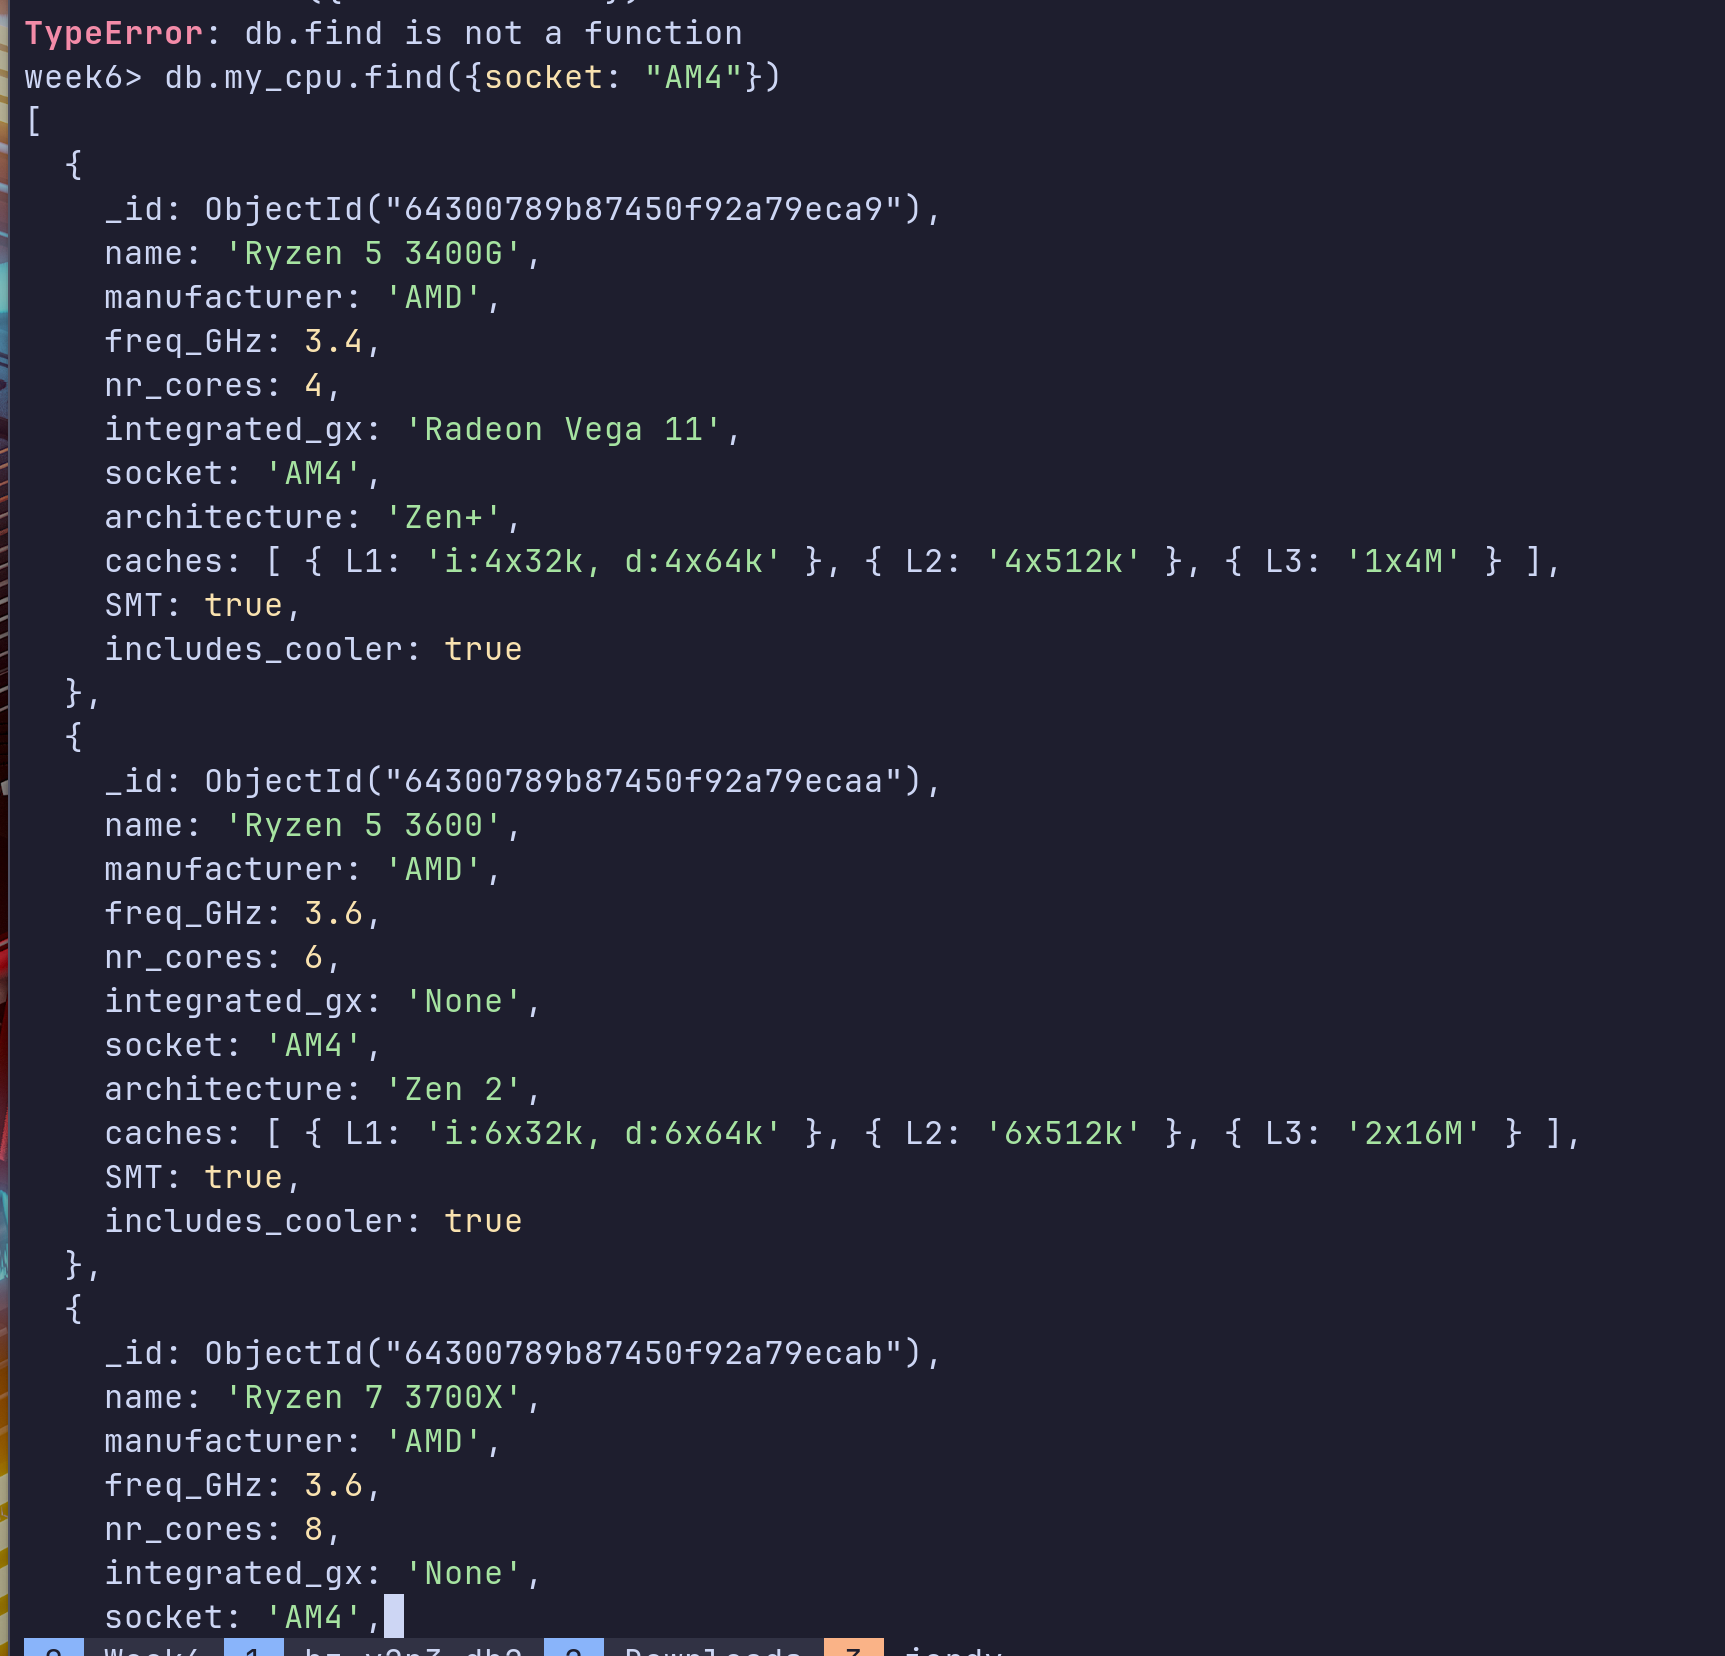
\includegraphics[height=\textheight,width=\textwidth,keepaspectratio]{question2a}
		\part
		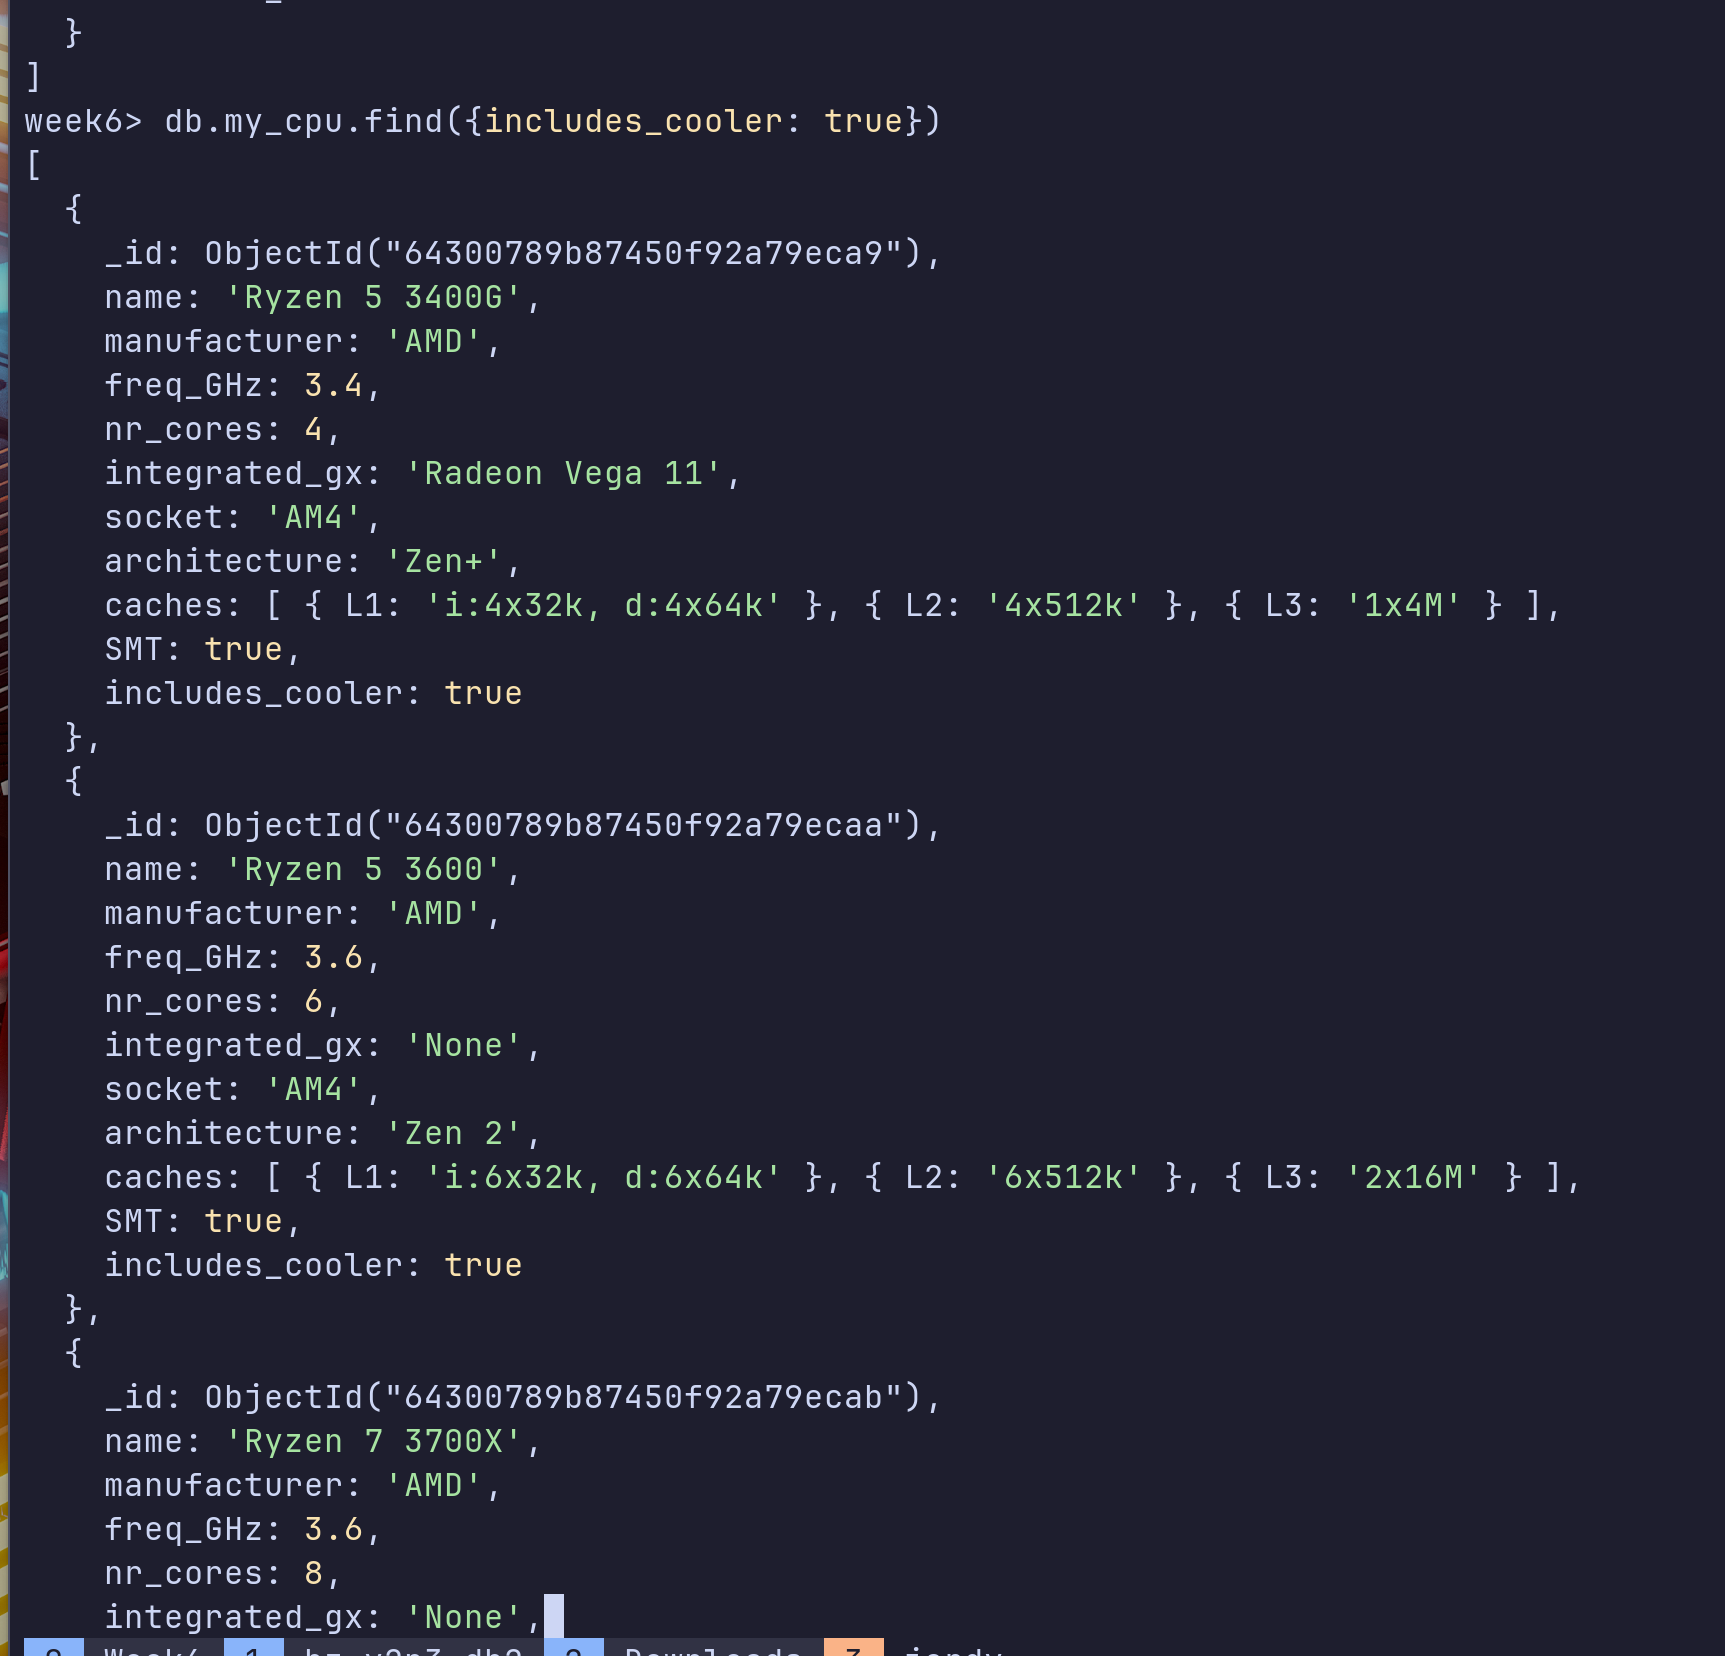
\includegraphics[height=\textheight,width=\textwidth,keepaspectratio]{question2b}
		\part
		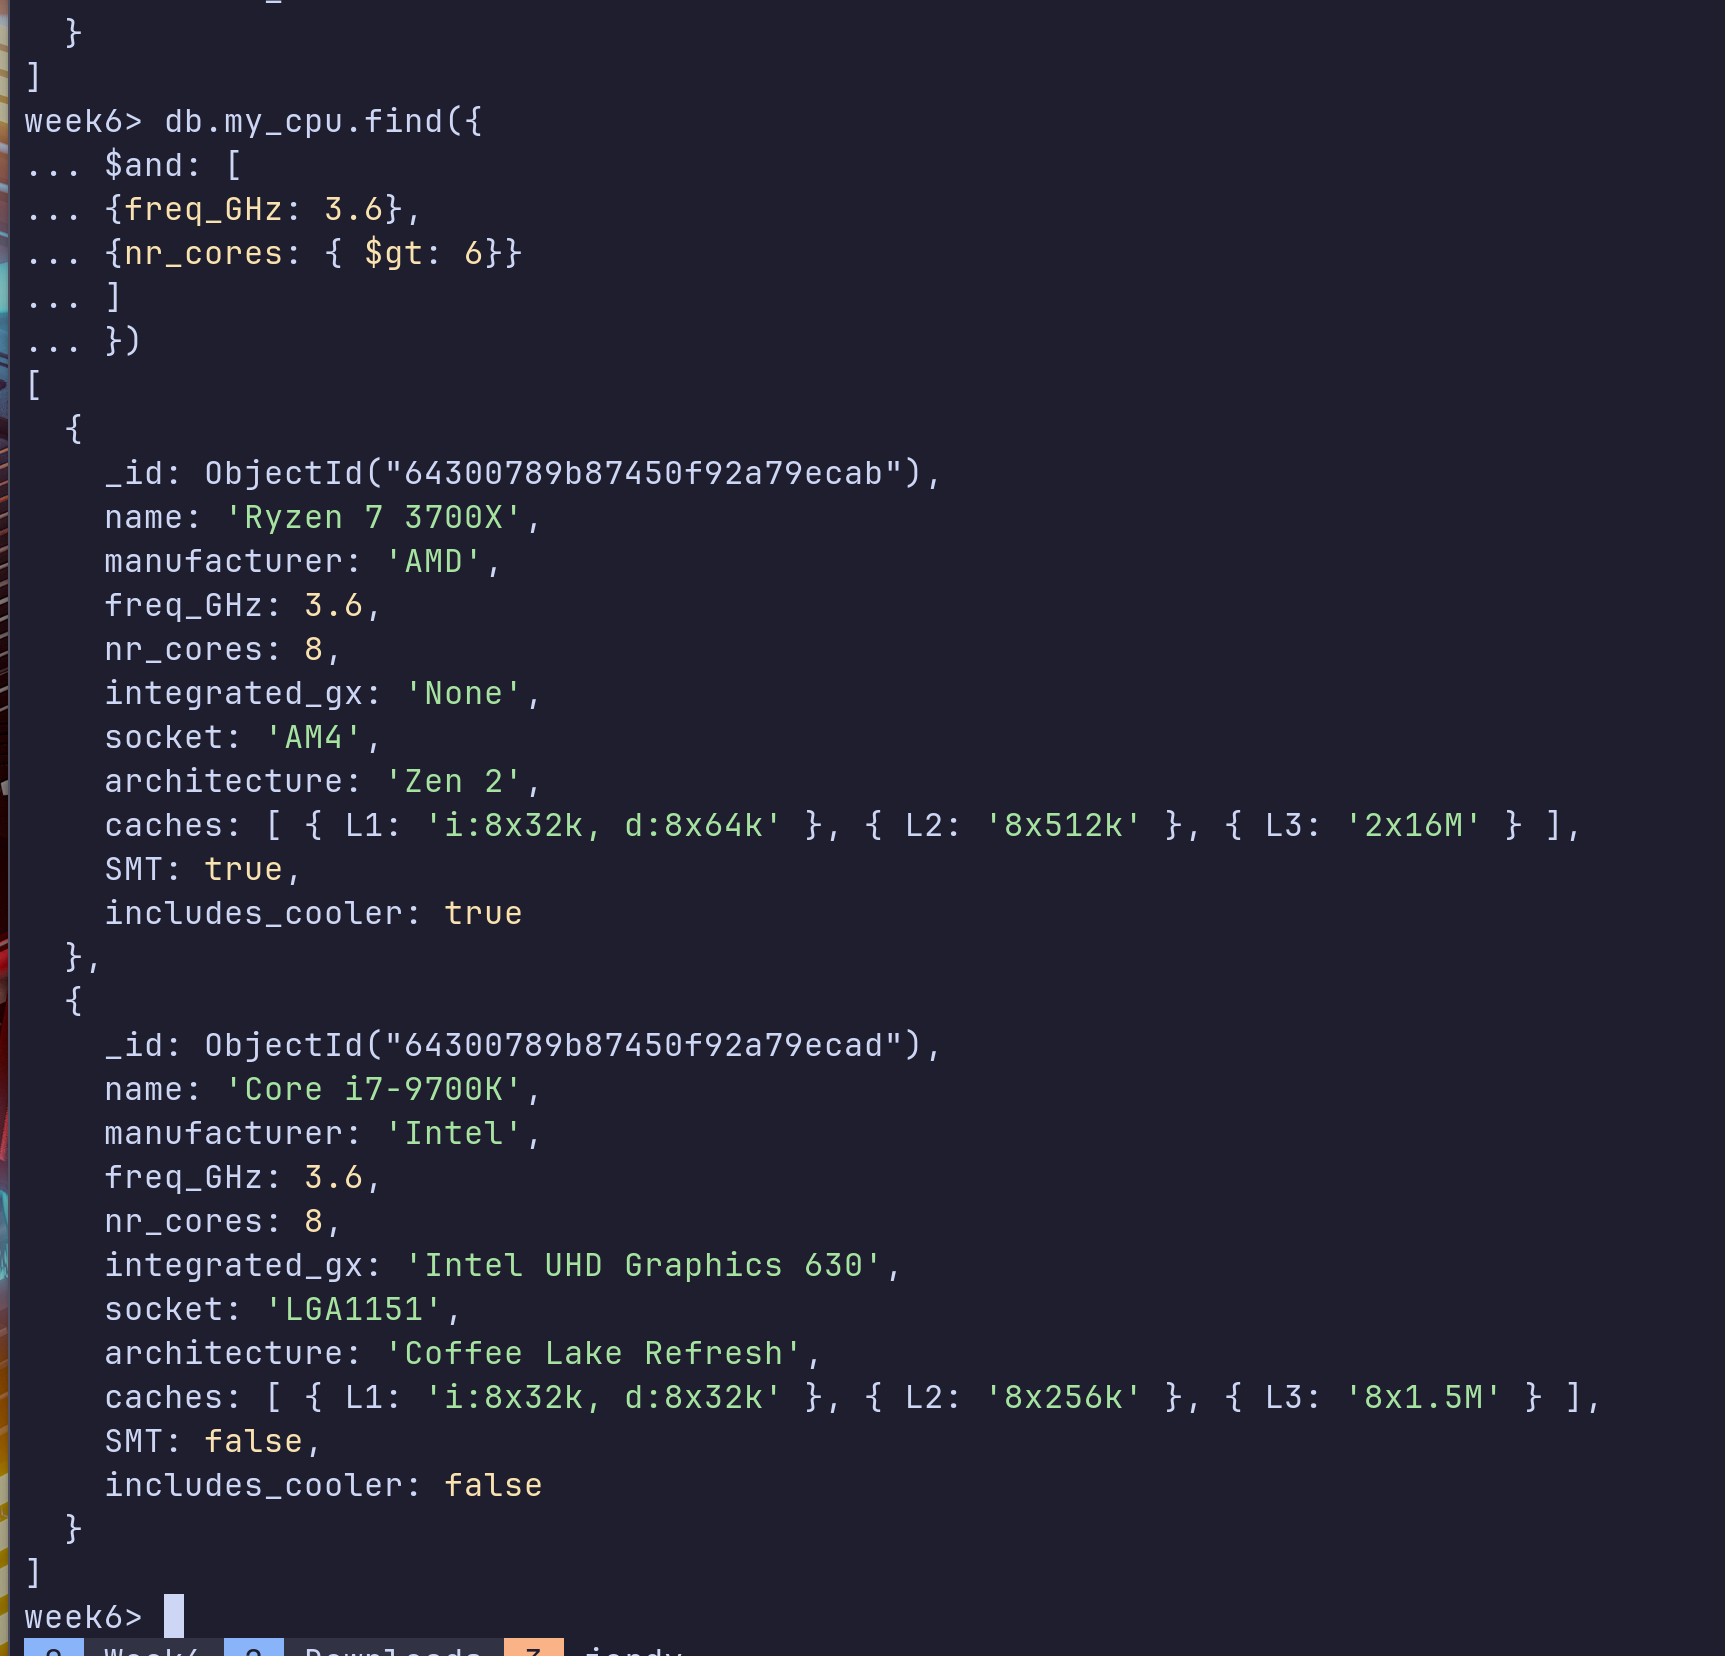
\includegraphics[height=\textheight,width=\textwidth,keepaspectratio]{question2c}
		\part
		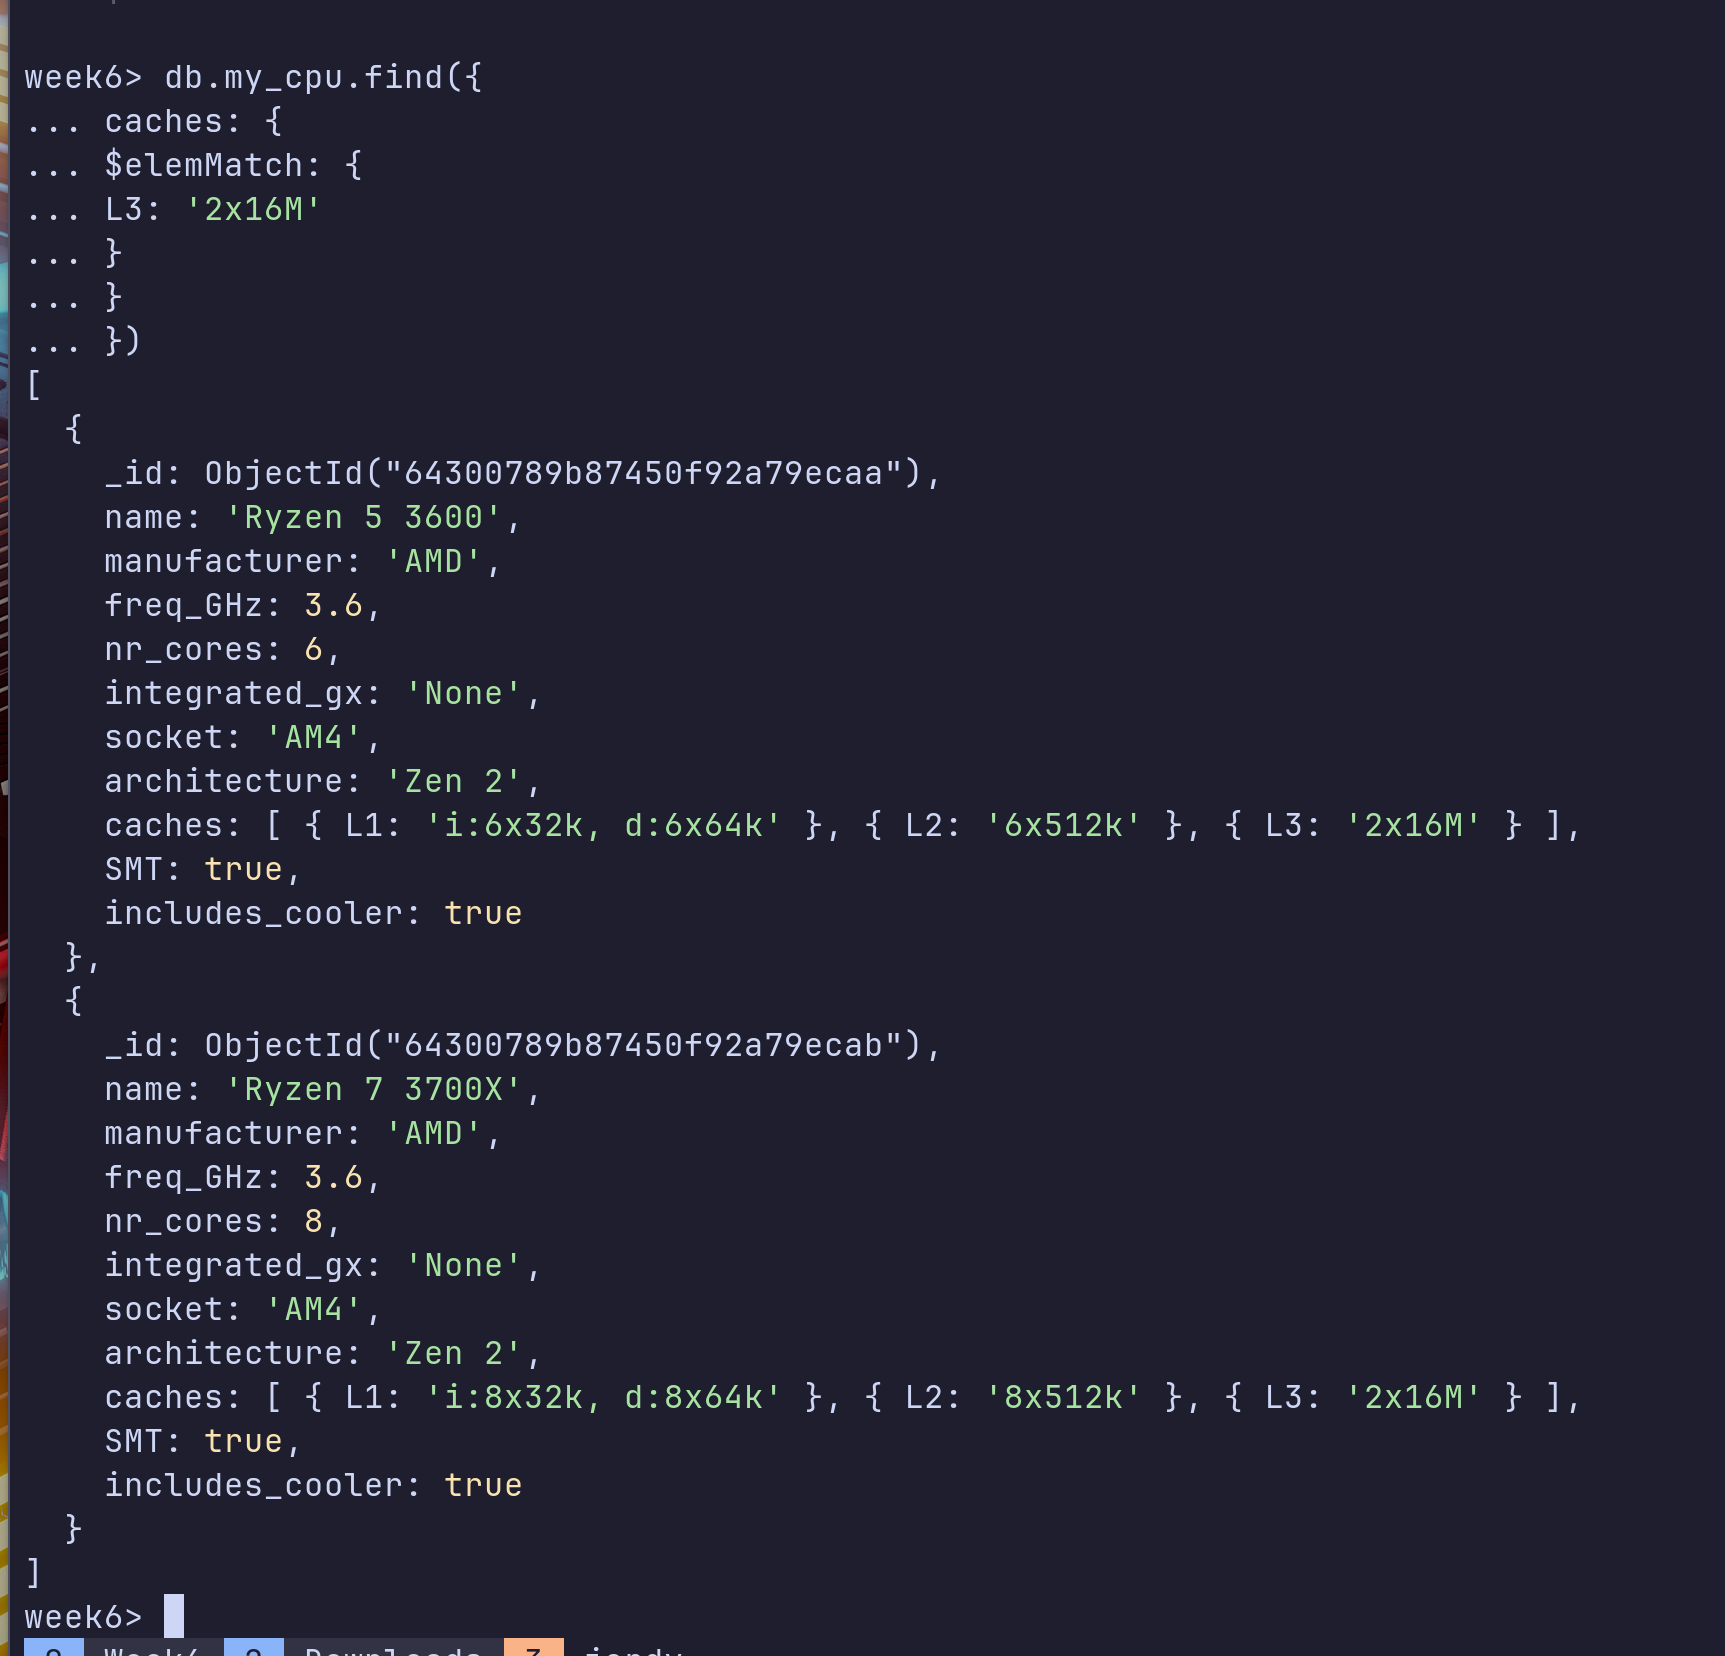
\includegraphics[height=\textheight,width=\textwidth,keepaspectratio]{question2d}
		\part
		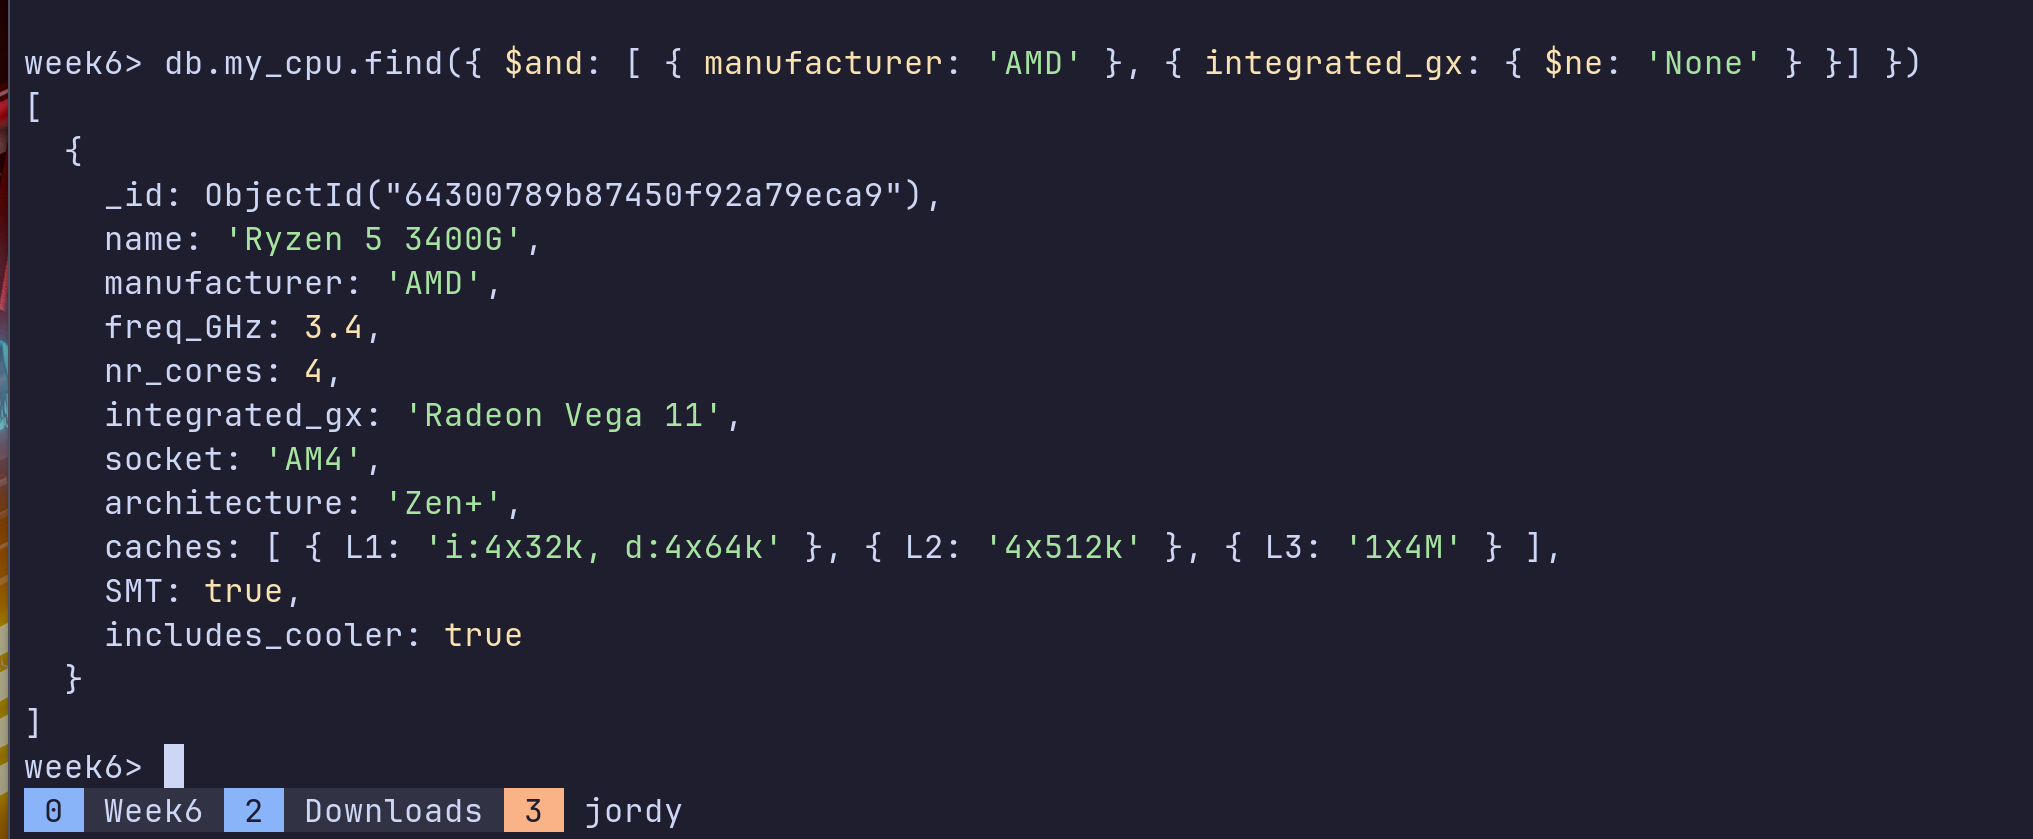
\includegraphics[height=\textheight,width=\textwidth,keepaspectratio]{question2e}
	\end{parts}
	\question
	\begin{parts}
		\part
		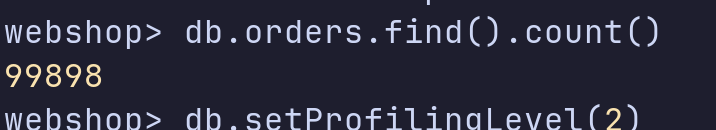
\includegraphics[keepaspectratio]{question3a}
		\part
		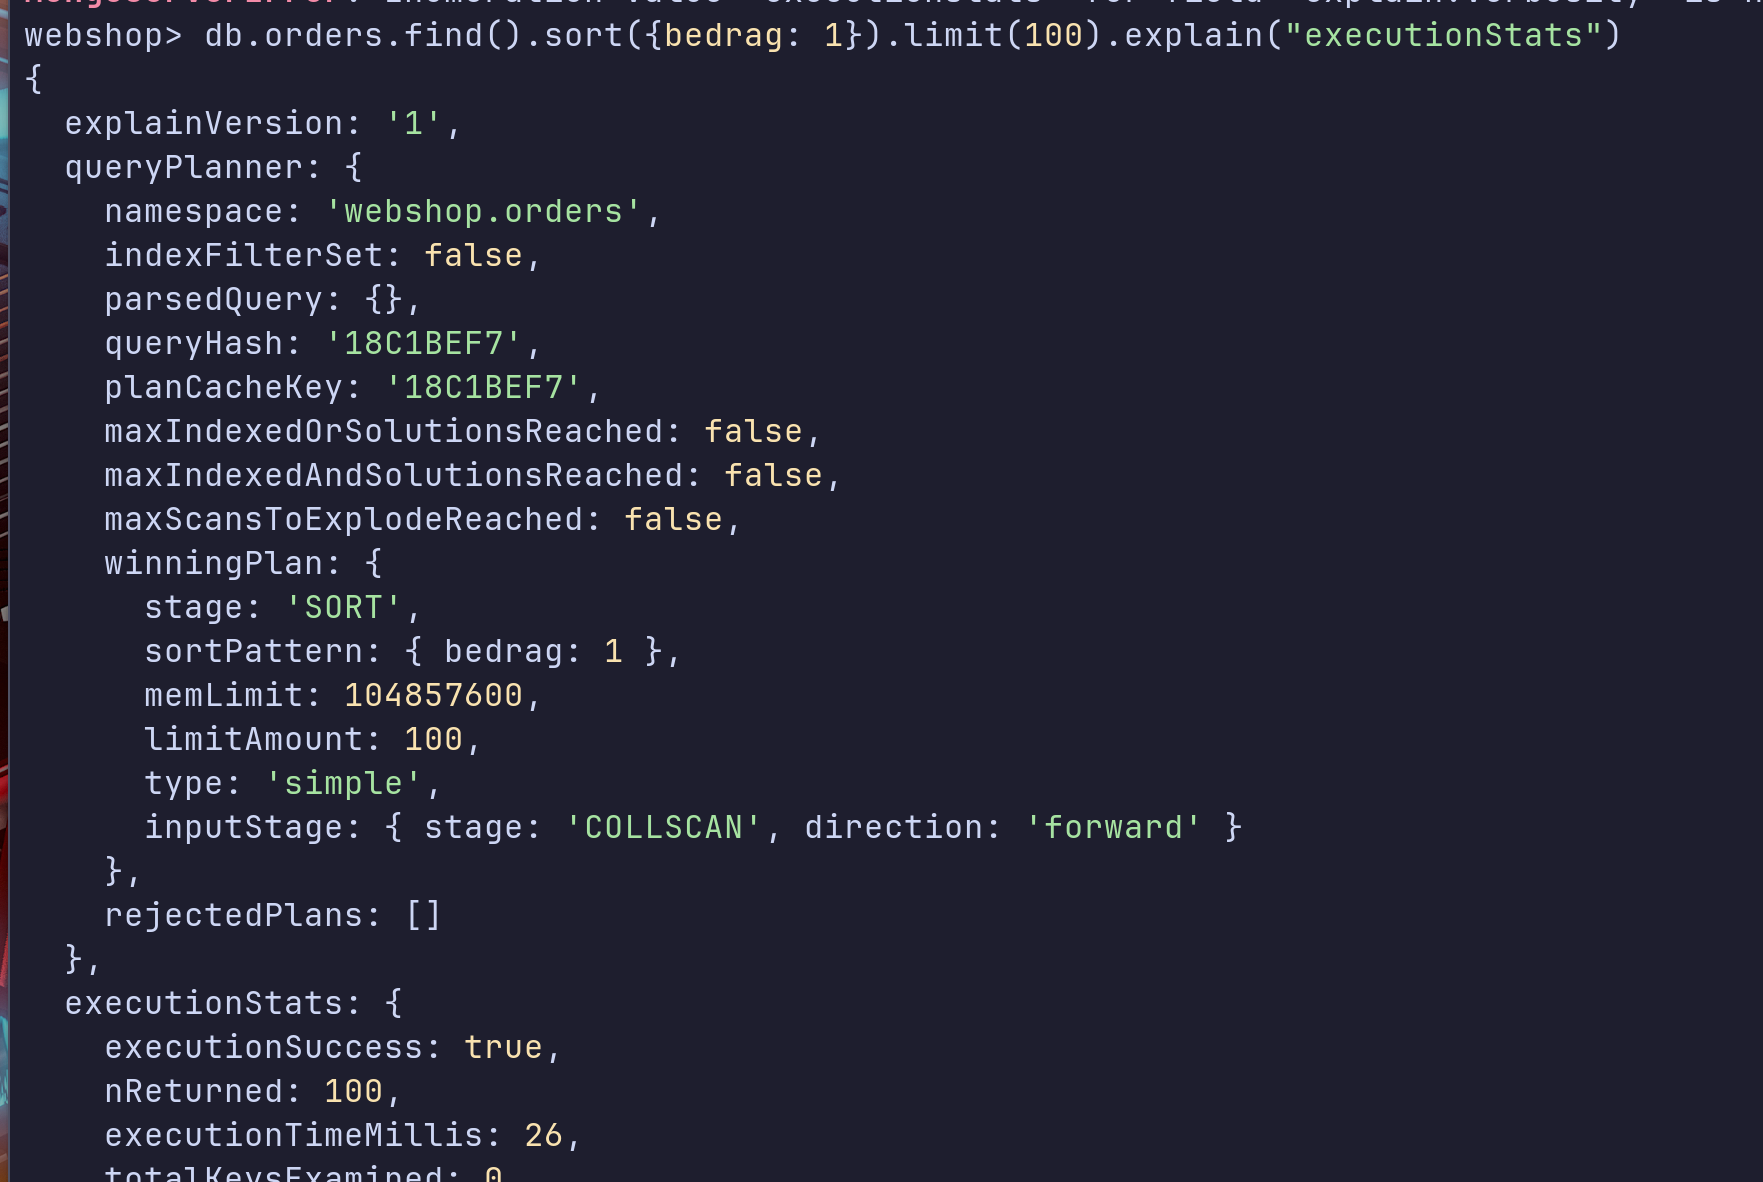
\includegraphics[height=\textheight,width=\textwidth,keepaspectratio]{question3b_1.png}
		26 ms


		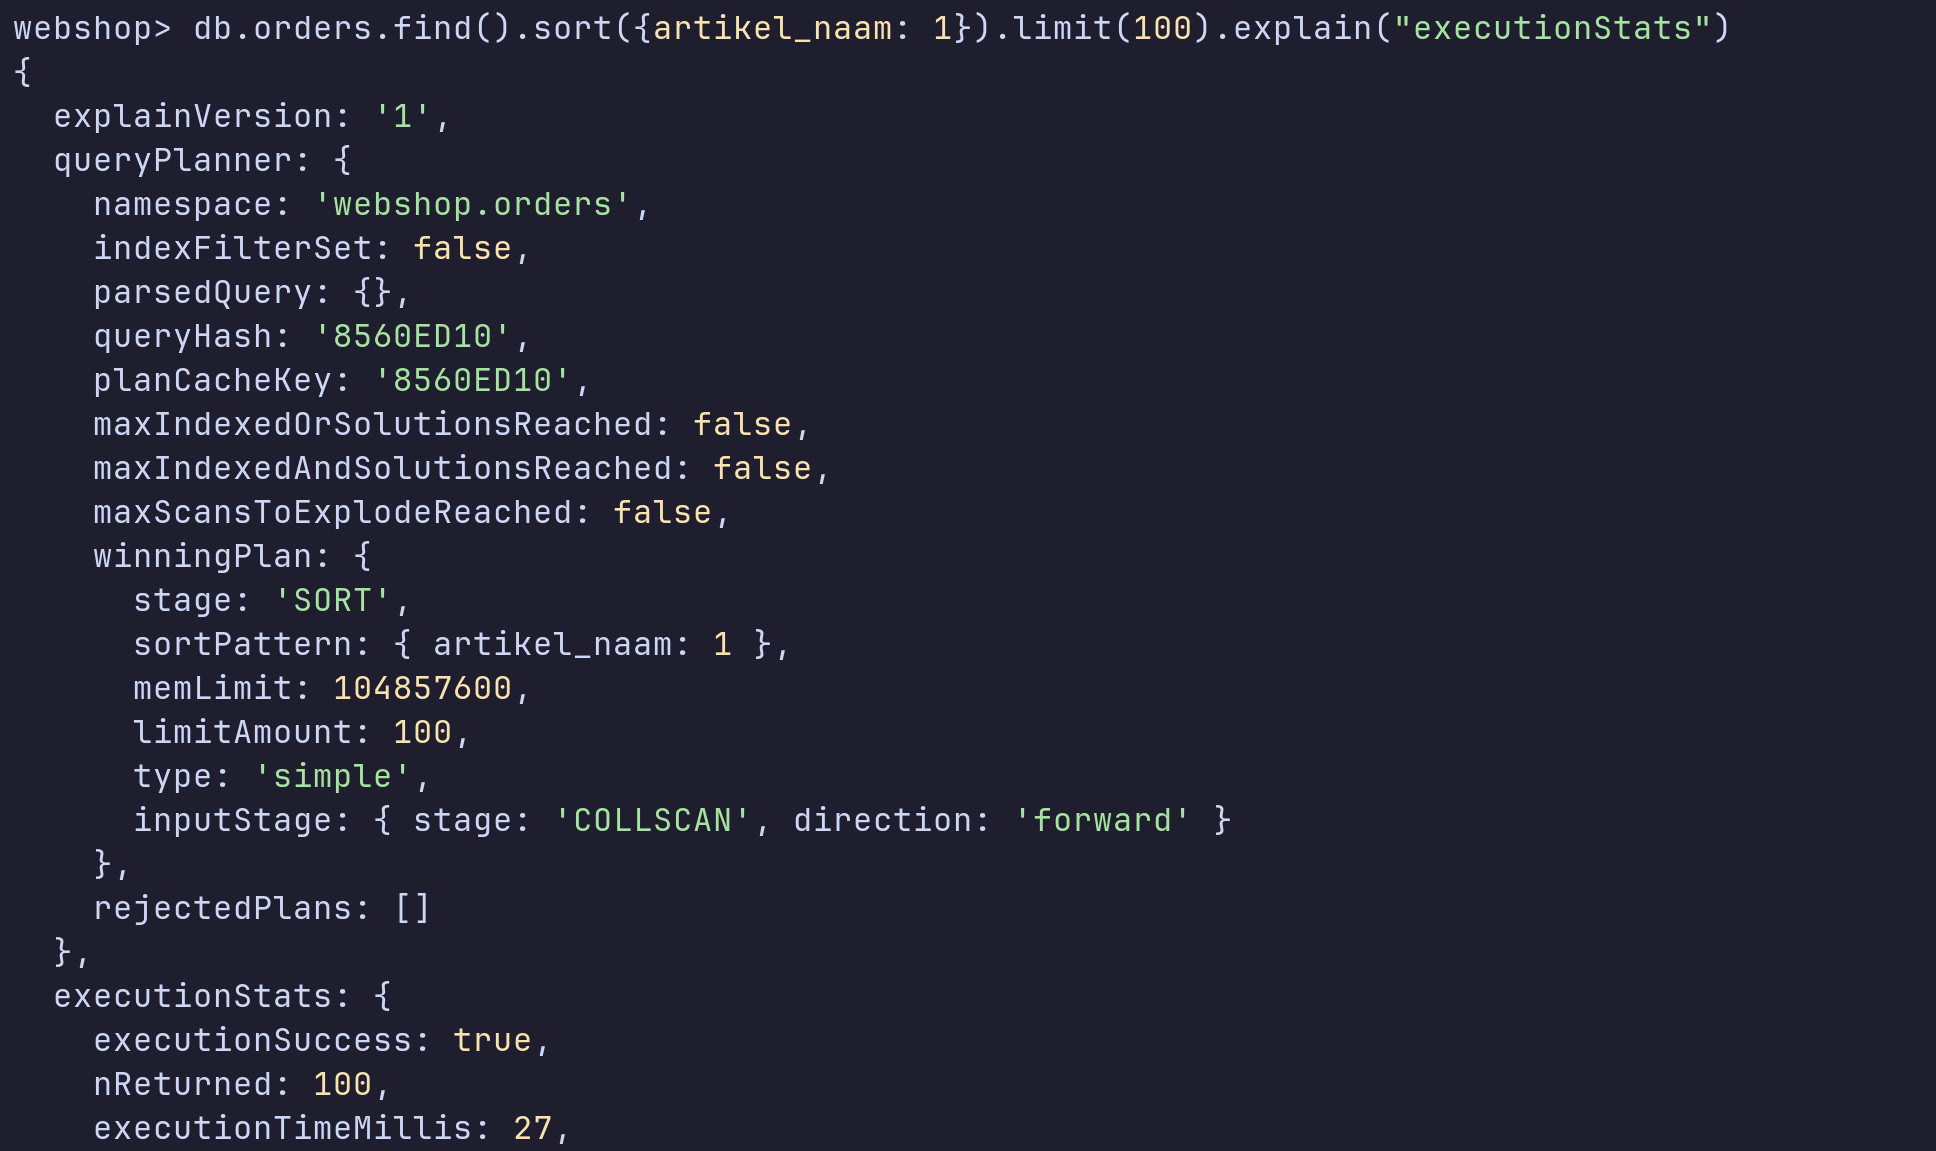
\includegraphics[height=\textheight,width=\textwidth,keepaspectratio]{question3b_2.png}
		27 ms
		\part
		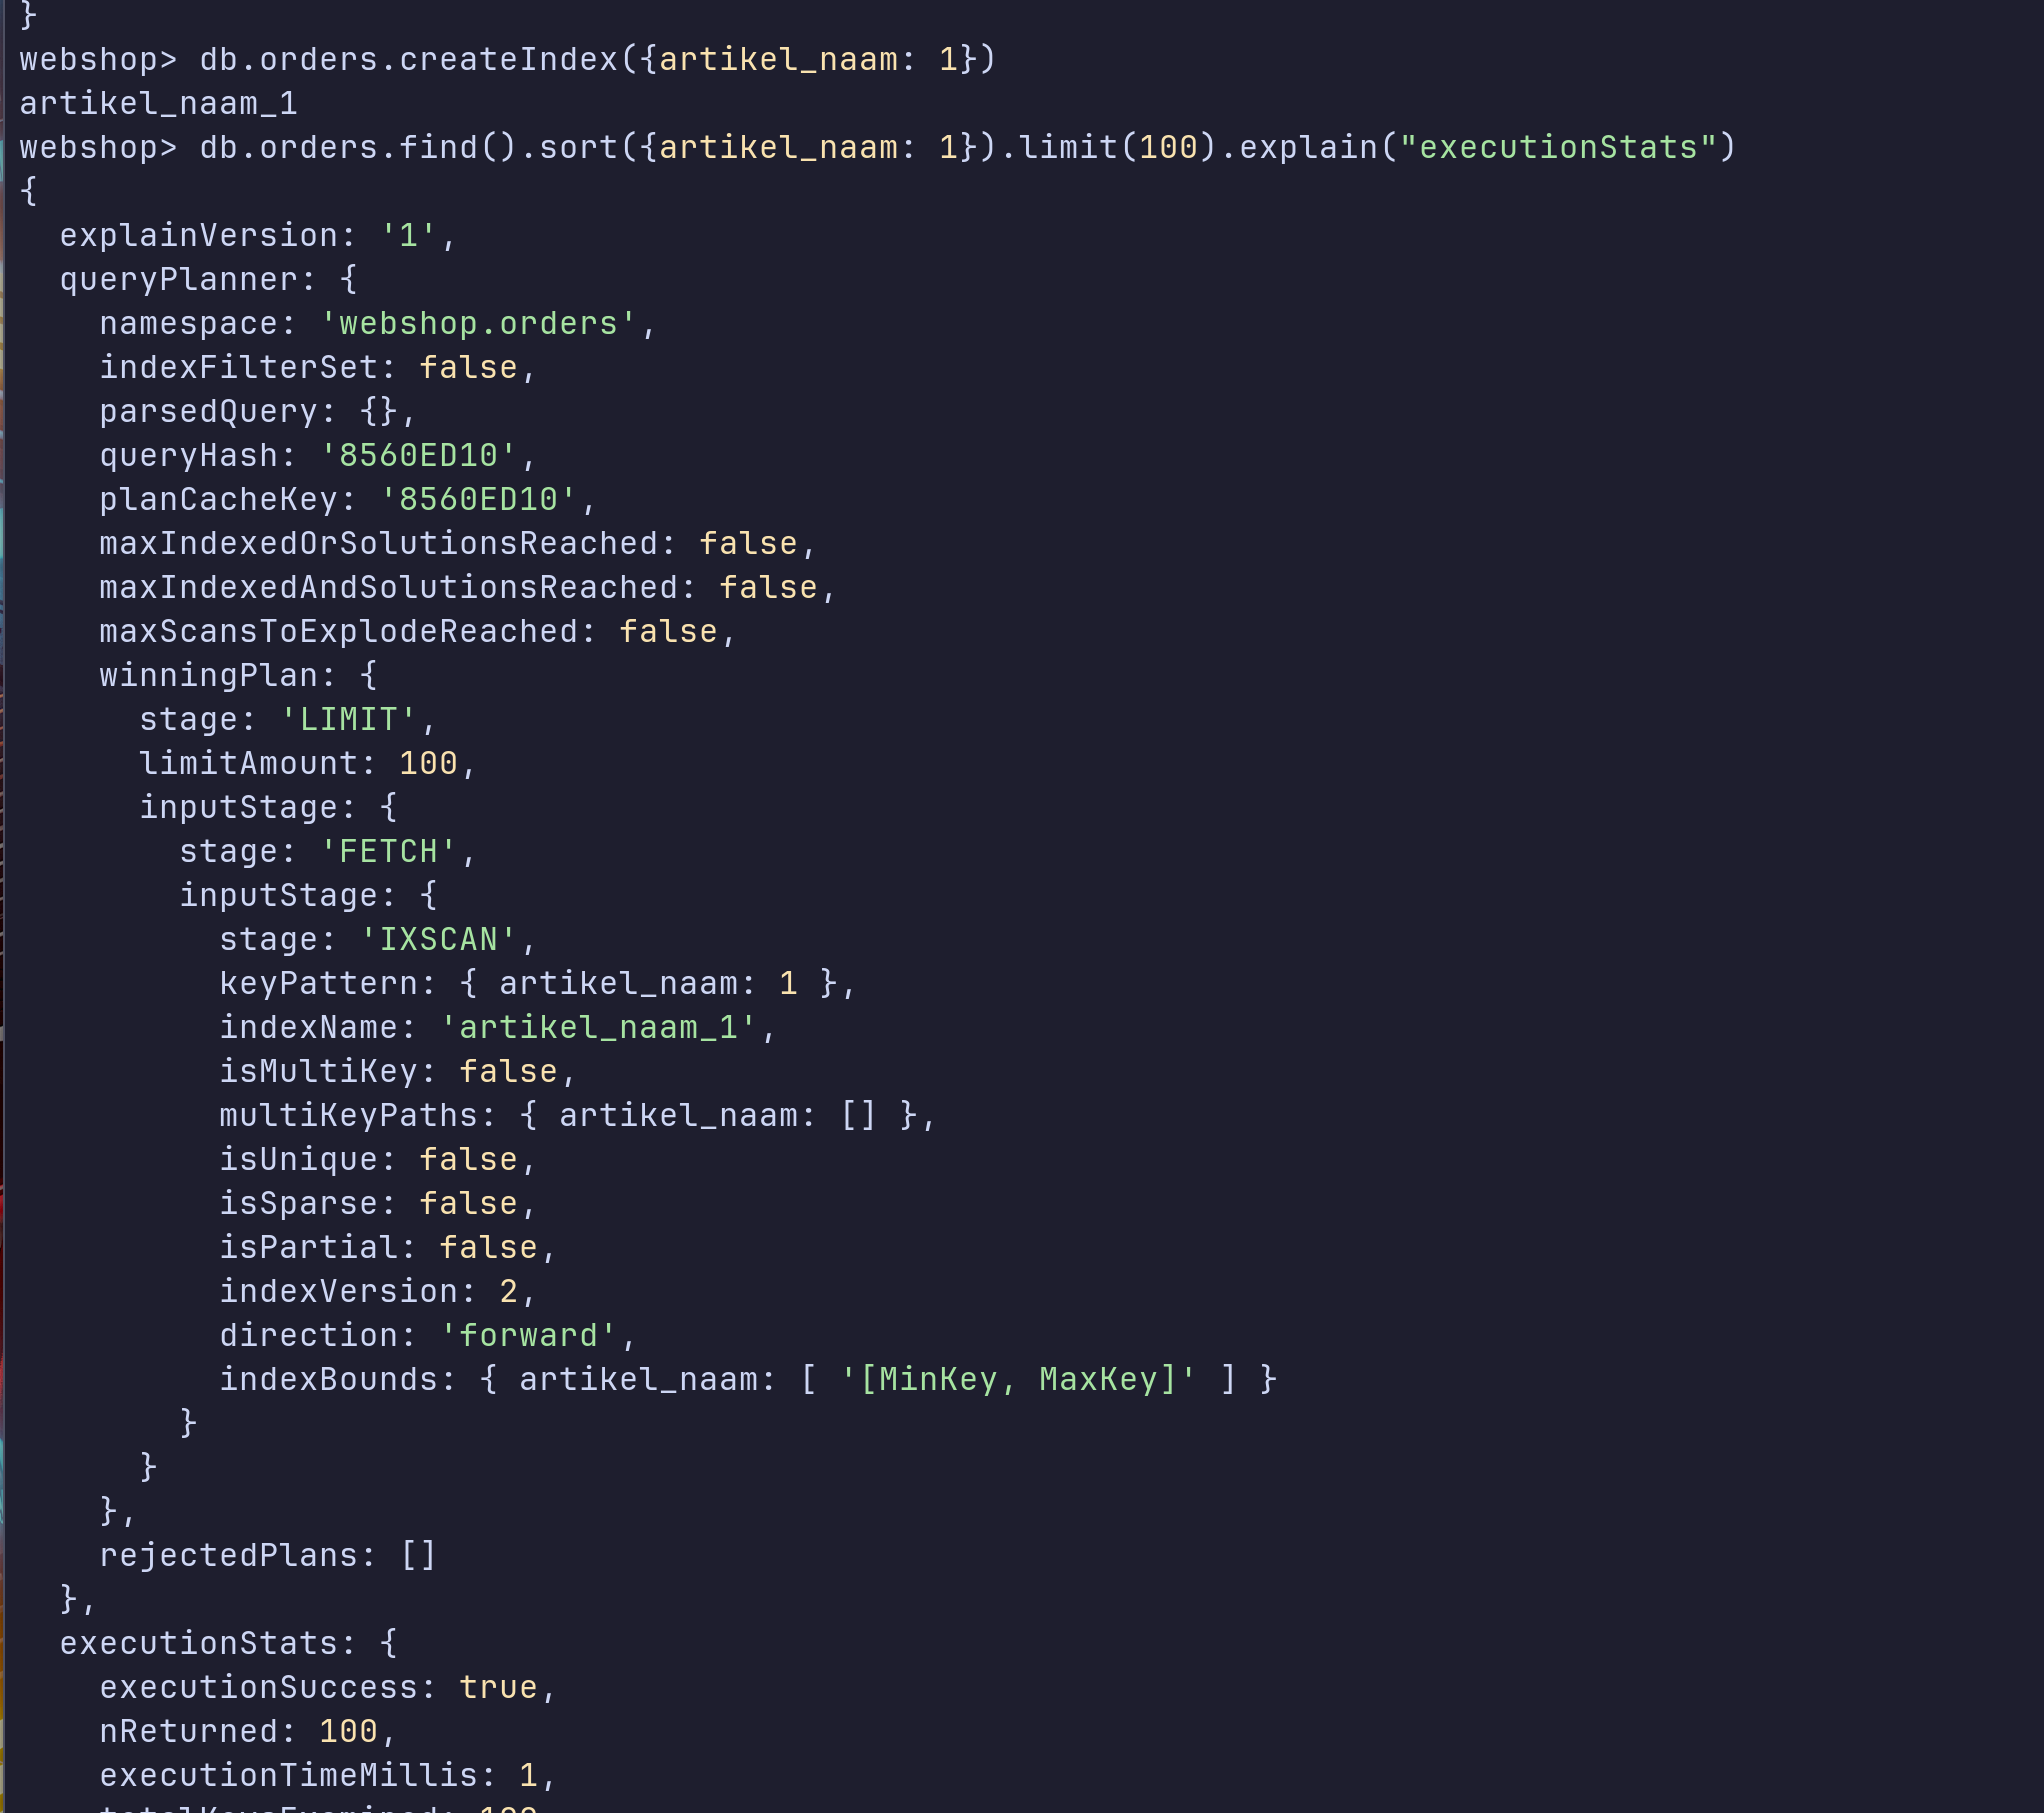
\includegraphics[height=\textheight,width=\textwidth,keepaspectratio]{question3c.png}
		1 ms
		\part
		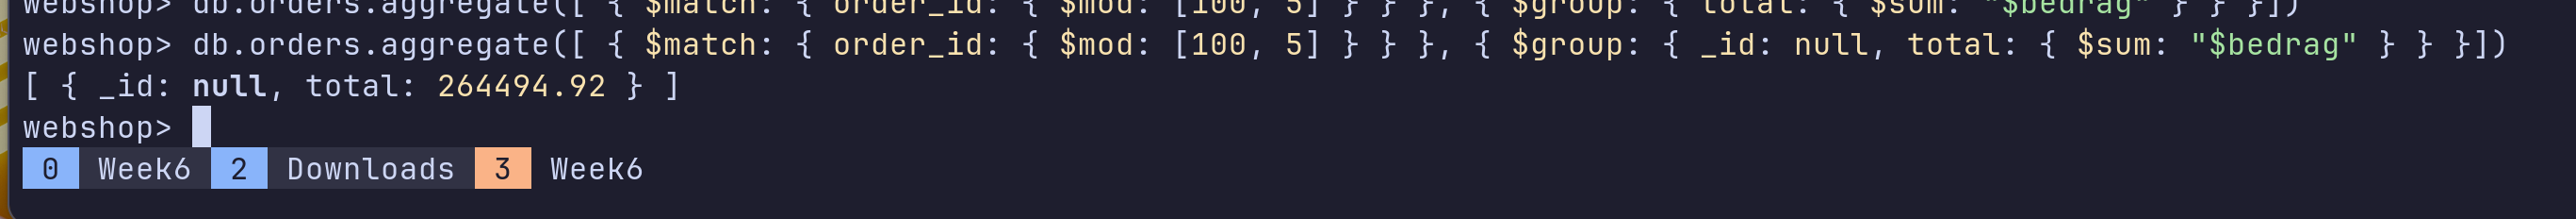
\includegraphics[height=\textheight,width=\textwidth,keepaspectratio]{question3d.png}
	\end{parts}
	\question
	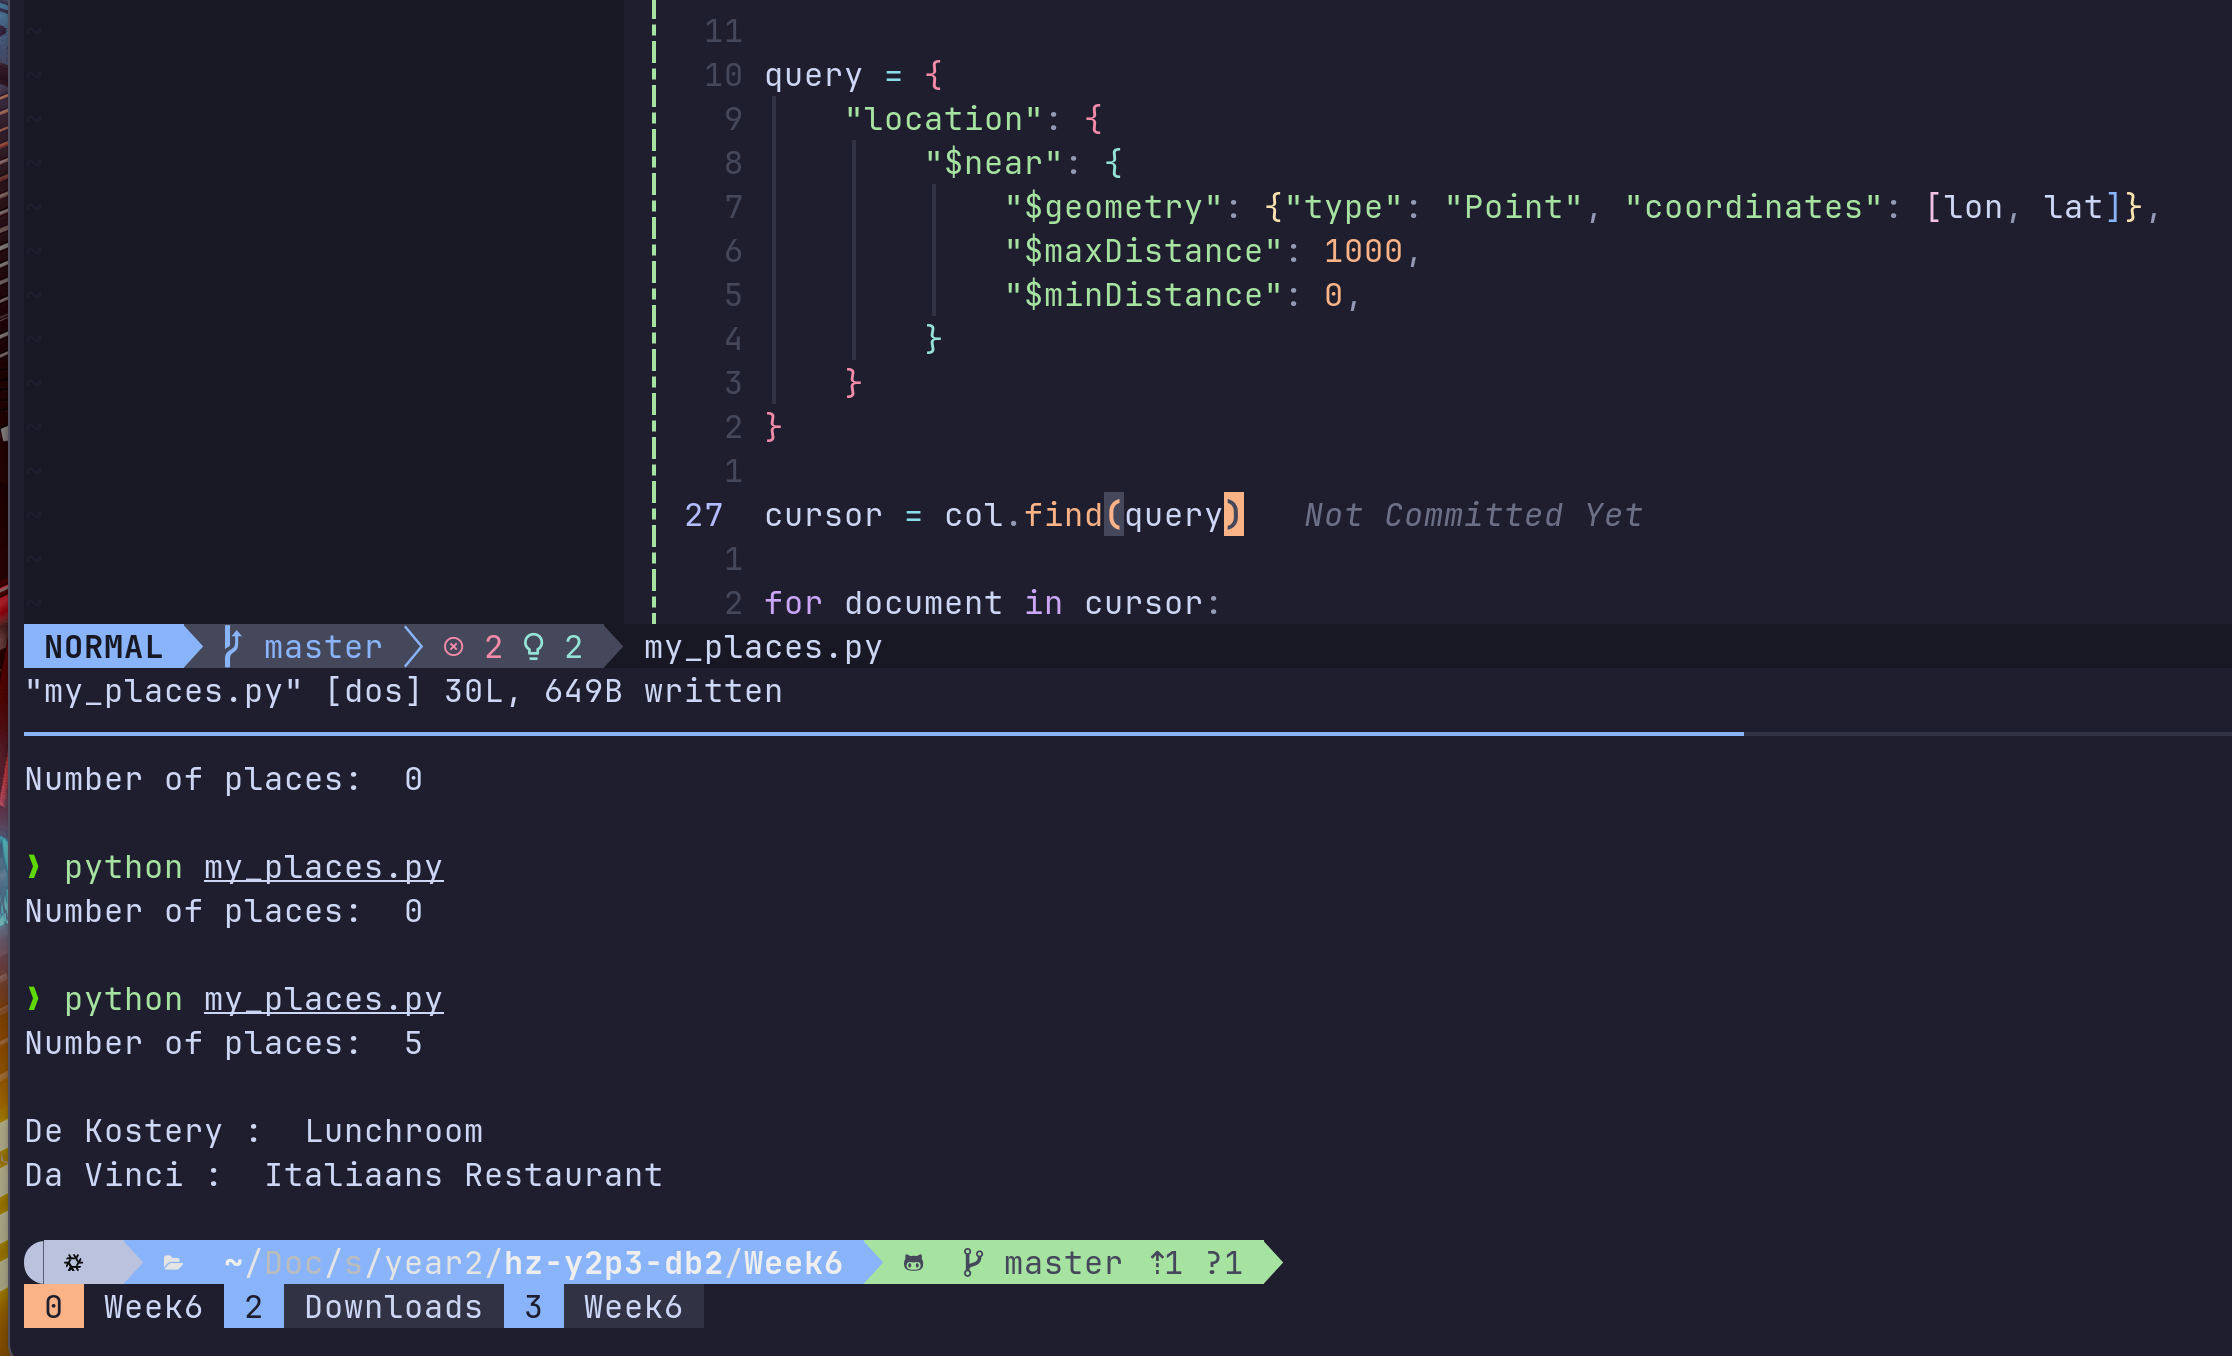
\includegraphics[height=\textheight,width=\textwidth,keepaspectratio]{question4.png}
	\question
	\begin{parts}
		\part
		\begin{itemize}
			\item
			      Alle films vinden met rating NC-17 of R en een title met FREAKY of TERMINATOR erin
			\item
			      Een lookup doen om category te joinen
			\item
			      Een lookup doen om actor te joinen
			\item
			      Een match doen om te zoeken op category name Horror of Sci-Fi
			\item
			      Een match doen op actor first name Uma
		\end{itemize}
		Dit alles in een aggregate function doen
	\end{parts}

\end{questions}

\end{document}
